\documentclass[journal,12pt,twocolumn]{IEEEtran}
\usepackage{setspace}
\usepackage{gensymb}
\usepackage{xcolor}
\usepackage{caption}
\singlespacing
\usepackage{siunitx}
\usepackage[cmex10]{amsmath}
\usepackage{mathtools}
\usepackage{hyperref}
\usepackage{amsthm}
\usepackage{mathrsfs}
\usepackage{txfonts}
\usepackage{stfloats}
\usepackage{cite}
\usepackage{cases}
\usepackage{subfig}
\usepackage{longtable}
\usepackage{multirow}
\usepackage{enumitem}
\usepackage{bm}
\usepackage{mathtools}
\usepackage{listings}
\usepackage{tikz}
\usetikzlibrary{shapes,arrows,positioning}
\usepackage{circuitikz}
\renewcommand{\vec}[1]{\boldsymbol{\mathbf{#1}}}
\DeclareMathOperator*{\Res}{Res}
\renewcommand\thesection{\arabic{section}}
\renewcommand\thesubsection{\thesection.\arabic{subsection}}
\renewcommand\thesubsubsection{\thesubsection.\arabic{subsubsection}}

\renewcommand\thesectiondis{\arabic{section}}
\renewcommand\thesubsectiondis{\thesectiondis.\arabic{subsection}}
\renewcommand\thesubsubsectiondis{\thesubsectiondis.\arabic{subsubsection}}
\hyphenation{op-tical net-works semi-conduc-tor}

\lstset{
language=Python,
frame=single, 
breaklines=true,
columns=fullflexible
}
\begin{document}
\theoremstyle{definition}
\newtheorem{theorem}{Theorem}[section]
\newtheorem{problem}{Problem}
\newtheorem{proposition}{Proposition}[section]
\newtheorem{lemma}{Lemma}[section]
\newtheorem{corollary}[theorem]{Corollary}
\newtheorem{example}{Example}[section]
\newtheorem{definition}{Definition}[section]
\newcommand{\BEQA}{\begin{eqnarray}}
        \newcommand{\EEQA}{\end{eqnarray}}
\newcommand{\define}{\stackrel{\triangle}{=}}
\newcommand{\myvec}[1]{\ensuremath{\begin{pmatrix}#1\end{pmatrix}}}
\newcommand{\mydet}[1]{\ensuremath{\begin{vmatrix}#1\end{vmatrix}}}
\bibliographystyle{IEEEtran}
\providecommand{\nCr}[2]{\,^{#1}C_{#2}} % nCr
\providecommand{\nPr}[2]{\,^{#1}P_{#2}} % nPr
\providecommand{\mbf}{\mathbf}
\providecommand{\pr}[1]{\ensuremath{\Pr\left(#1\right)}}
\providecommand{\qfunc}[1]{\ensuremath{Q\left(#1\right)}}
\providecommand{\sbrak}[1]{\ensuremath{{}\left[#1\right]}}
\providecommand{\lsbrak}[1]{\ensuremath{{}\left[#1\right.}}
\providecommand{\rsbrak}[1]{\ensuremath{{}\left.#1\right]}}
\providecommand{\brak}[1]{\ensuremath{\left(#1\right)}}
\providecommand{\lbrak}[1]{\ensuremath{\left(#1\right.}}
\providecommand{\rbrak}[1]{\ensuremath{\left.#1\right)}}
\providecommand{\cbrak}[1]{\ensuremath{\left\{#1\right\}}}
\providecommand{\lcbrak}[1]{\ensuremath{\left\{#1\right.}}
\providecommand{\rcbrak}[1]{\ensuremath{\left.#1\right\}}}
\theoremstyle{remark}
\newtheorem{rem}{Remark}
\newcommand{\sgn}{\mathop{\mathrm{sgn}}}
\newcommand{\rect}{\mathop{\mathrm{rect}}}
\newcommand{\sinc}{\mathop{\mathrm{sinc}}}
\providecommand{\abs}[1]{\left\vert#1\right\vert}
\providecommand{\res}[1]{\Res\displaylimits_{#1}}
\providecommand{\norm}[1]{\lVert#1\rVert}
\providecommand{\mtx}[1]{\mathbf{#1}}
\providecommand{\mean}[1]{E\left[ #1 \right]}
\providecommand{\fourier}{\overset{\mathcal{F}}{ \rightleftharpoons}}
\providecommand{\ztrans}{\overset{\mathcal{Z}}{ \rightleftharpoons}}
\providecommand{\system}[1]{\overset{\mathcal{#1}}{ \longleftrightarrow}}
\newcommand{\solution}{\noindent \textbf{Solution: }}
\providecommand{\dec}[2]{\ensuremath{\overset{#1}{\underset{#2}{\gtrless}}}}
\let\StandardTheFigure\thefigure
\def\putbox#1#2#3{\makebox[0in][l]{\makebox[#1][l]{}\raisebox{\baselineskip}[0in][0in]{\raisebox{#2}[0in][0in]{#3}}}}
\def\rightbox#1{\makebox[0in][r]{#1}}
\def\centbox#1{\makebox[0in]{#1}}
\def\topbox#1{\raisebox{-\baselineskip}[0in][0in]{#1}}
\def\midbox#1{\raisebox{-0.5\baselineskip}[0in][0in]{#1}}

\vspace{3cm}
\title{11.11.3.5}
\author{Lokesh Surana}
\maketitle
\section*{Class 11, Chapter 11, Exercise 3.5}
Q. Find the coordinates of the focii, the vertices, the length of major and minor axes, the eccentricity and the length of the latus rectum of an ellipse whose equation is given by $\frac{x^2}{49}+\frac{y^2}{36}=1$.

\solution The given equation of ellipse can be rearranged as
\begin{align}
    36x^2+49y^2-1764=0\label{eq:1}
\end{align}

The above equation can be equated to the general equation of conic sections
\begin{align}
 g\brak{\vec{x}}=\vec{x}^\top \vec{V} \vec{x} + 2\vec{u}^\top \vec{x} + f = 0\label{eq:2}
\end{align}

From \eqref{eq:1} and \eqref{eq:2}
\begin{align}
 \vec{V} &= \myvec{36&0\\0&49}\label{eq:3}\\
 \vec{u} &= \vec{0}\\
 f &= -1764
\end{align}

From \eqref{eq:3} the eigen values $\lambda_1 \text{ and } \lambda_2$ are given as
\begin{align}
 \lambda_1 &= 36\\
 \lambda_2 &= 49
\end{align}

Since the given matrix $\vec{V}$ is diagonal, the Eigen vector matrix will be identity. It is given as
\begin{align}
	\vec{P} &= \myvec{\vec{p}_1 & \vec{p}_2}\\
		&= \myvec{1&0\\0&1}
\end{align}

\begin{enumerate}
\item The eccentricity of the ellipse is given as
\begin{align}
	e &= \sqrt{1 - \frac{\lambda_1}{\lambda_2}} = \sqrt{1-\frac{36}{49}}\\
	  &= \frac{\sqrt{13}}{7}
\end{align}
\item Finding the coordinates of Focii
\begin{align}
	\vec{n} &= \sqrt{\lambda_2}\vec{p}_1= \sqrt{49} \myvec{7\\0}\\
	&= \myvec{0\\5}
\end{align}
\begin{align}
	\label{eq:4}
	c &= \frac{e\vec{u}^\top \vec{n} \pm \sqrt{e^2 \brak{\vec{u}^\top \vec{n}}^2-\lambda_1 \brak{e^2 -1}\brak{\norm{\vec{u}}^2-\lambda_1 f}}}{\lambda_1 e\brak{e^2-1}}
\end{align}

Substituting values of $e,\vec{u},\vec{n},\lambda_1 \text{ and } f$ in \eqref{eq:4}
\begin{align}
	c &= \frac{0 \pm \sqrt{0-49\brak{\frac{13}{49}-1}\brak{0+49\brak{1764}}}}{49\frac{\sqrt{13}}{7}\brak{\frac{13}{49}-1}}\\
	&= \frac{\pm 343}{\sqrt{13}}
\end{align}
The focus $\vec{F}$ of the ellipse is expressed as
\begin{align}
	\vec{F} &= \frac{ce^2 \vec{n}-\vec{u}}{\lambda_1}\\
	&= \frac{\pm \frac{343}{\sqrt{13}}\brak{\frac{13}{49}}\myvec{7\\0}}{49}\\
	&= \myvec{\pm \sqrt{13}\\0}
\end{align}
\item The length of the major axis is given by
\begin{align}
	\label{eq:5}
	&2\sqrt{\abs{\frac{f_0}{\lambda_1}}}\\
	f_0 &= \vec{u}^\top \vec{V}^{-1} \vec{u} -f\\
	    &= 1764\\
	\eqref{eq:5} &\implies 2\sqrt{\abs{\frac{1764}{36}}}
	 = 14
\end{align}
\item The length of minor axis is given by
\begin{align}
	2\sqrt{\abs{\frac{f_0}{\lambda_2}}}&= 2\sqrt{\abs{\frac{1764}{49}}}\\
	&= 12
\end{align}
\item The vertices of the ellipse are given by
\begin{align}
	\pm \myvec{\sqrt{\abs{\frac{f_0}{\lambda_1}}}\\0}= \pm \myvec{7\\0}
\end{align}
\item The length of latus rectum is given as
\begin{align}
	2\frac{\sqrt{\abs{f_0 \lambda_1}}}{\lambda_2} &= 2\frac{\sqrt{\abs{1764\brak{36}}}}{49}\\
	&= \frac{72}{7}
\end{align}
\end{enumerate}

\begin{figure}[!htb]
    \centering
    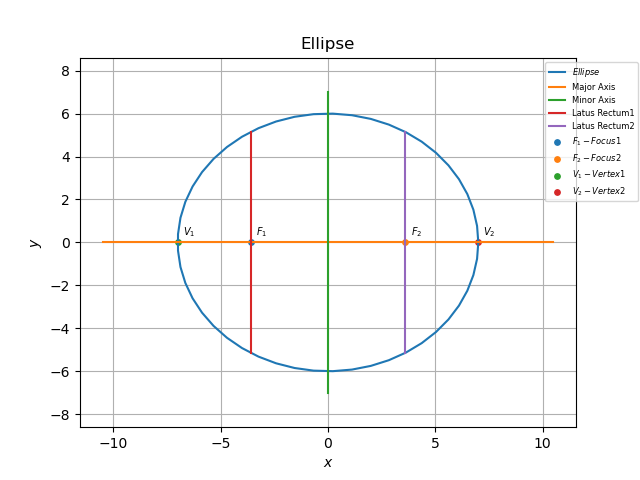
\includegraphics[width=\columnwidth]{figs/ellipse.png}
    \caption{ellipse}
    \label{fig:ellipse}
\end{figure}


\end{document}